\batchmode
\documentclass[a4paper]{book}
\usepackage{makeidx}
\usepackage{natbib}
\usepackage{graphicx}
\usepackage{multicol}
\usepackage{float}
\usepackage{listings}
\usepackage{color}
\usepackage{ifthen}
\usepackage[table]{xcolor}
\usepackage{textcomp}
\usepackage{alltt}
\usepackage[utf8]{inputenc}
\usepackage{mathptmx}
\usepackage[scaled=.90]{helvet}
\usepackage{courier}
\usepackage{sectsty}
\usepackage[titles]{tocloft}
\usepackage{doxygen}
\lstset{language=C++,inputencoding=utf8,basicstyle=\footnotesize,breaklines=true,breakatwhitespace=true,tabsize=8,numbers=left }
\makeindex
\setcounter{tocdepth}{3}
\renewcommand{\footrulewidth}{0.4pt}
\renewcommand{\familydefault}{\sfdefault}
\hfuzz=15pt
\setlength{\emergencystretch}{15pt}
\hbadness=750
\tolerance=750
\begin{document}
\begin{titlepage}
\vspace*{7cm}
\begin{center}
{\Large rsg\-\_\-urdfloader }\\
\vspace*{1cm}
{\large \-Generated by Doxygen 1.7.6.1}\\
\vspace*{0.5cm}
{\small Mon Feb 24 2014 13:54:22}\\
\end{center}
\end{titlepage}
\clearemptydoublepage
\pagenumbering{roman}
\tableofcontents
\clearemptydoublepage
\pagenumbering{arabic}
\chapter{\-Namespace \-Index}
\section{\-Namespace \-List}
\-Here is a list of all namespaces with brief descriptions\-:\begin{DoxyCompactList}
\item\contentsline{section}{{\bf rsg\-\_\-urdfloader} }{\pageref{namespacersg__urdfloader}}{}
\end{DoxyCompactList}

\chapter{\-Class \-Index}
\section{\-Class \-List}
\-Here are the classes, structs, unions and interfaces with brief descriptions\-:\begin{DoxyCompactList}
\item\contentsline{section}{{\bf rsg\-\_\-urdfloader\-::\-U\-R\-D\-Fto\-R\-S\-G} }{\pageref{classrsg__urdfloader_1_1URDFtoRSG}}{}
\end{DoxyCompactList}

\chapter{\-File \-Index}
\section{\-File \-List}
\-Here is a list of all files with brief descriptions\-:\begin{DoxyCompactList}
\item\contentsline{section}{{\bf rsg\-\_\-urdfloader.\-cpp} }{\pageref{rsg__urdfloader_8cpp}}{}
\item\contentsline{section}{{\bf rsg\-\_\-urdfloader.\-h} }{\pageref{rsg__urdfloader_8h}}{}
\item\contentsline{section}{{\bf test.\-cpp} }{\pageref{test_8cpp}}{}
\end{DoxyCompactList}

\chapter{\-Namespace \-Documentation}
\section{rsg\-\_\-urdfloader \-Namespace \-Reference}
\label{namespacersg__urdfloader}\index{rsg\-\_\-urdfloader@{rsg\-\_\-urdfloader}}
\subsection*{\-Classes}
\begin{DoxyCompactItemize}
\item 
class {\bf \-U\-R\-D\-Fto\-R\-S\-G}
\end{DoxyCompactItemize}

\chapter{\-Class \-Documentation}
\section{rsg\-\_\-urdfloader\-:\-:\-U\-R\-D\-Fto\-R\-S\-G \-Class \-Reference}
\label{classrsg__urdfloader_1_1URDFtoRSG}\index{rsg\-\_\-urdfloader\-::\-U\-R\-D\-Fto\-R\-S\-G@{rsg\-\_\-urdfloader\-::\-U\-R\-D\-Fto\-R\-S\-G}}


{\ttfamily \#include $<$rsg\-\_\-urdfloader.\-h$>$}

\subsection*{\-Public \-Member \-Functions}
\begin{DoxyCompactItemize}
\item 
bool {\bf rsg\-From\-File} (const string \&file)
\item 
bool {\bf rsg\-From\-Param} (const string \&param)
\item 
bool {\bf rsg\-From\-String} (const string \&xml)
\item 
bool {\bf rsg\-From\-Urdf\-Model} (const urdf\-::\-Model\-Interface \&robot\-\_\-model)
\item 
bool {\bf rsg\-From\-Xml} (\-Ti\-Xml\-Document $\ast$xml\-\_\-doc)
\item 
{\bf \-U\-R\-D\-Fto\-R\-S\-G} ()
\item 
bool {\bf visualize} ()
\item 
{\bf $\sim$\-U\-R\-D\-Fto\-R\-S\-G} ()
\end{DoxyCompactItemize}
\subsection*{\-Public \-Attributes}
\begin{DoxyCompactItemize}
\item 
\-World\-Model $\ast$ {\bf wm}
\end{DoxyCompactItemize}
\subsection*{\-Private \-Member \-Functions}
\begin{DoxyCompactItemize}
\item 
bool {\bf add\-Children\-To\-R\-S\-G} (boost\-::shared\-\_\-ptr$<$ const urdf\-::\-Link $>$ root, rsg\-::\-Id id)
\item 
bool {\bf add\-Geometry} ()
\item 
vector$<$ rsg\-::\-Attribute $>$ {\bf add\-Joint} (boost\-::shared\-\_\-ptr$<$ urdf\-::\-Joint $>$ jnt)
\item 
vector$<$ rsg\-::\-Attribute $>$ {\bf add\-Mass\-Properties} (boost\-::shared\-\_\-ptr$<$ const urdf\-::\-Link $>$ link)
\end{DoxyCompactItemize}


\subsection{\-Detailed \-Description}


\-Definition at line 35 of file rsg\-\_\-urdfloader.\-h.



\subsection{\-Constructor \& \-Destructor \-Documentation}
\index{rsg\-\_\-urdfloader\-::\-U\-R\-D\-Fto\-R\-S\-G@{rsg\-\_\-urdfloader\-::\-U\-R\-D\-Fto\-R\-S\-G}!\-U\-R\-D\-Fto\-R\-S\-G@{\-U\-R\-D\-Fto\-R\-S\-G}}
\index{\-U\-R\-D\-Fto\-R\-S\-G@{\-U\-R\-D\-Fto\-R\-S\-G}!rsg_urdfloader::URDFtoRSG@{rsg\-\_\-urdfloader\-::\-U\-R\-D\-Fto\-R\-S\-G}}
\subsubsection[{\-U\-R\-D\-Fto\-R\-S\-G}]{\setlength{\rightskip}{0pt plus 5cm}{\bf rsg\-\_\-urdfloader\-::\-U\-R\-D\-Fto\-R\-S\-G\-::\-U\-R\-D\-Fto\-R\-S\-G} (
\begin{DoxyParamCaption}
{}
\end{DoxyParamCaption}
)\hspace{0.3cm}{\ttfamily  [inline]}}\label{classrsg__urdfloader_1_1URDFtoRSG_a3bc8b1fbc41971f604bd9d9cd4545a09}


\-Definition at line 40 of file rsg\-\_\-urdfloader.\-h.

\index{rsg\-\_\-urdfloader\-::\-U\-R\-D\-Fto\-R\-S\-G@{rsg\-\_\-urdfloader\-::\-U\-R\-D\-Fto\-R\-S\-G}!$\sim$\-U\-R\-D\-Fto\-R\-S\-G@{$\sim$\-U\-R\-D\-Fto\-R\-S\-G}}
\index{$\sim$\-U\-R\-D\-Fto\-R\-S\-G@{$\sim$\-U\-R\-D\-Fto\-R\-S\-G}!rsg_urdfloader::URDFtoRSG@{rsg\-\_\-urdfloader\-::\-U\-R\-D\-Fto\-R\-S\-G}}
\subsubsection[{$\sim$\-U\-R\-D\-Fto\-R\-S\-G}]{\setlength{\rightskip}{0pt plus 5cm}{\bf rsg\-\_\-urdfloader\-::\-U\-R\-D\-Fto\-R\-S\-G\-::$\sim$\-U\-R\-D\-Fto\-R\-S\-G} (
\begin{DoxyParamCaption}
{}
\end{DoxyParamCaption}
)\hspace{0.3cm}{\ttfamily  [inline]}}\label{classrsg__urdfloader_1_1URDFtoRSG_a4b58018552edab4257e811e7d8dd87da}


\-Definition at line 45 of file rsg\-\_\-urdfloader.\-h.



\subsection{\-Member \-Function \-Documentation}
\index{rsg\-\_\-urdfloader\-::\-U\-R\-D\-Fto\-R\-S\-G@{rsg\-\_\-urdfloader\-::\-U\-R\-D\-Fto\-R\-S\-G}!add\-Children\-To\-R\-S\-G@{add\-Children\-To\-R\-S\-G}}
\index{add\-Children\-To\-R\-S\-G@{add\-Children\-To\-R\-S\-G}!rsg_urdfloader::URDFtoRSG@{rsg\-\_\-urdfloader\-::\-U\-R\-D\-Fto\-R\-S\-G}}
\subsubsection[{add\-Children\-To\-R\-S\-G}]{\setlength{\rightskip}{0pt plus 5cm}bool {\bf \-U\-R\-D\-Fto\-R\-S\-G\-::add\-Children\-To\-R\-S\-G} (
\begin{DoxyParamCaption}
\item[{boost\-::shared\-\_\-ptr$<$ const urdf\-::\-Link $>$}]{root, }
\item[{rsg\-::\-Id}]{id}
\end{DoxyParamCaption}
)\hspace{0.3cm}{\ttfamily  [private]}}\label{classrsg__urdfloader_1_1URDFtoRSG_a171cee8009f284a47e07a7ad1110ba9a}


\-Definition at line 21 of file rsg\-\_\-urdfloader.\-cpp.

\index{rsg\-\_\-urdfloader\-::\-U\-R\-D\-Fto\-R\-S\-G@{rsg\-\_\-urdfloader\-::\-U\-R\-D\-Fto\-R\-S\-G}!add\-Geometry@{add\-Geometry}}
\index{add\-Geometry@{add\-Geometry}!rsg_urdfloader::URDFtoRSG@{rsg\-\_\-urdfloader\-::\-U\-R\-D\-Fto\-R\-S\-G}}
\subsubsection[{add\-Geometry}]{\setlength{\rightskip}{0pt plus 5cm}bool {\bf rsg\-\_\-urdfloader\-::\-U\-R\-D\-Fto\-R\-S\-G\-::add\-Geometry} (
\begin{DoxyParamCaption}
{}
\end{DoxyParamCaption}
)\hspace{0.3cm}{\ttfamily  [private]}}\label{classrsg__urdfloader_1_1URDFtoRSG_aca11ac5f1162319b199e3744cff1194e}
\index{rsg\-\_\-urdfloader\-::\-U\-R\-D\-Fto\-R\-S\-G@{rsg\-\_\-urdfloader\-::\-U\-R\-D\-Fto\-R\-S\-G}!add\-Joint@{add\-Joint}}
\index{add\-Joint@{add\-Joint}!rsg_urdfloader::URDFtoRSG@{rsg\-\_\-urdfloader\-::\-U\-R\-D\-Fto\-R\-S\-G}}
\subsubsection[{add\-Joint}]{\setlength{\rightskip}{0pt plus 5cm}vector$<$ rsg\-::\-Attribute $>$ {\bf \-U\-R\-D\-Fto\-R\-S\-G\-::add\-Joint} (
\begin{DoxyParamCaption}
\item[{boost\-::shared\-\_\-ptr$<$ urdf\-::\-Joint $>$}]{jnt}
\end{DoxyParamCaption}
)\hspace{0.3cm}{\ttfamily  [private]}}\label{classrsg__urdfloader_1_1URDFtoRSG_a29ebacf54db9f8abbd6126ad860e2315}


\-Definition at line 57 of file rsg\-\_\-urdfloader.\-cpp.

\index{rsg\-\_\-urdfloader\-::\-U\-R\-D\-Fto\-R\-S\-G@{rsg\-\_\-urdfloader\-::\-U\-R\-D\-Fto\-R\-S\-G}!add\-Mass\-Properties@{add\-Mass\-Properties}}
\index{add\-Mass\-Properties@{add\-Mass\-Properties}!rsg_urdfloader::URDFtoRSG@{rsg\-\_\-urdfloader\-::\-U\-R\-D\-Fto\-R\-S\-G}}
\subsubsection[{add\-Mass\-Properties}]{\setlength{\rightskip}{0pt plus 5cm}vector$<$rsg\-::\-Attribute$>$ {\bf rsg\-\_\-urdfloader\-::\-U\-R\-D\-Fto\-R\-S\-G\-::add\-Mass\-Properties} (
\begin{DoxyParamCaption}
\item[{boost\-::shared\-\_\-ptr$<$ const urdf\-::\-Link $>$}]{link}
\end{DoxyParamCaption}
)\hspace{0.3cm}{\ttfamily  [private]}}\label{classrsg__urdfloader_1_1URDFtoRSG_ac45d09b43a73cc5fb794061883ed92ad}
\index{rsg\-\_\-urdfloader\-::\-U\-R\-D\-Fto\-R\-S\-G@{rsg\-\_\-urdfloader\-::\-U\-R\-D\-Fto\-R\-S\-G}!rsg\-From\-File@{rsg\-From\-File}}
\index{rsg\-From\-File@{rsg\-From\-File}!rsg_urdfloader::URDFtoRSG@{rsg\-\_\-urdfloader\-::\-U\-R\-D\-Fto\-R\-S\-G}}
\subsubsection[{rsg\-From\-File}]{\setlength{\rightskip}{0pt plus 5cm}bool {\bf rsg\-\_\-urdfloader\-::\-U\-R\-D\-Fto\-R\-S\-G\-::rsg\-From\-File} (
\begin{DoxyParamCaption}
\item[{const string \&}]{file}
\end{DoxyParamCaption}
)\hspace{0.3cm}{\ttfamily  [inline]}}\label{classrsg__urdfloader_1_1URDFtoRSG_a77a1a7db31d893df7d47cba83f6d7b04}


\-Definition at line 63 of file rsg\-\_\-urdfloader.\-h.

\index{rsg\-\_\-urdfloader\-::\-U\-R\-D\-Fto\-R\-S\-G@{rsg\-\_\-urdfloader\-::\-U\-R\-D\-Fto\-R\-S\-G}!rsg\-From\-Param@{rsg\-From\-Param}}
\index{rsg\-From\-Param@{rsg\-From\-Param}!rsg_urdfloader::URDFtoRSG@{rsg\-\_\-urdfloader\-::\-U\-R\-D\-Fto\-R\-S\-G}}
\subsubsection[{rsg\-From\-Param}]{\setlength{\rightskip}{0pt plus 5cm}bool {\bf rsg\-\_\-urdfloader\-::\-U\-R\-D\-Fto\-R\-S\-G\-::rsg\-From\-Param} (
\begin{DoxyParamCaption}
\item[{const string \&}]{param}
\end{DoxyParamCaption}
)\hspace{0.3cm}{\ttfamily  [inline]}}\label{classrsg__urdfloader_1_1URDFtoRSG_aed39fa3297ce38d946ca0407cc5f4bc9}


\-Definition at line 71 of file rsg\-\_\-urdfloader.\-h.

\index{rsg\-\_\-urdfloader\-::\-U\-R\-D\-Fto\-R\-S\-G@{rsg\-\_\-urdfloader\-::\-U\-R\-D\-Fto\-R\-S\-G}!rsg\-From\-String@{rsg\-From\-String}}
\index{rsg\-From\-String@{rsg\-From\-String}!rsg_urdfloader::URDFtoRSG@{rsg\-\_\-urdfloader\-::\-U\-R\-D\-Fto\-R\-S\-G}}
\subsubsection[{rsg\-From\-String}]{\setlength{\rightskip}{0pt plus 5cm}bool {\bf rsg\-\_\-urdfloader\-::\-U\-R\-D\-Fto\-R\-S\-G\-::rsg\-From\-String} (
\begin{DoxyParamCaption}
\item[{const string \&}]{xml}
\end{DoxyParamCaption}
)\hspace{0.3cm}{\ttfamily  [inline]}}\label{classrsg__urdfloader_1_1URDFtoRSG_ab1a52a06fee5c6200941c8e7829a5fef}


\-Definition at line 81 of file rsg\-\_\-urdfloader.\-h.

\index{rsg\-\_\-urdfloader\-::\-U\-R\-D\-Fto\-R\-S\-G@{rsg\-\_\-urdfloader\-::\-U\-R\-D\-Fto\-R\-S\-G}!rsg\-From\-Urdf\-Model@{rsg\-From\-Urdf\-Model}}
\index{rsg\-From\-Urdf\-Model@{rsg\-From\-Urdf\-Model}!rsg_urdfloader::URDFtoRSG@{rsg\-\_\-urdfloader\-::\-U\-R\-D\-Fto\-R\-S\-G}}
\subsubsection[{rsg\-From\-Urdf\-Model}]{\setlength{\rightskip}{0pt plus 5cm}bool {\bf \-U\-R\-D\-Fto\-R\-S\-G\-::rsg\-From\-Urdf\-Model} (
\begin{DoxyParamCaption}
\item[{const urdf\-::\-Model\-Interface \&}]{robot\-\_\-model}
\end{DoxyParamCaption}
)}\label{classrsg__urdfloader_1_1URDFtoRSG_ad89d5ddb0a354eaf5de2c35580fd928b}


\-Definition at line 10 of file rsg\-\_\-urdfloader.\-cpp.

\index{rsg\-\_\-urdfloader\-::\-U\-R\-D\-Fto\-R\-S\-G@{rsg\-\_\-urdfloader\-::\-U\-R\-D\-Fto\-R\-S\-G}!rsg\-From\-Xml@{rsg\-From\-Xml}}
\index{rsg\-From\-Xml@{rsg\-From\-Xml}!rsg_urdfloader::URDFtoRSG@{rsg\-\_\-urdfloader\-::\-U\-R\-D\-Fto\-R\-S\-G}}
\subsubsection[{rsg\-From\-Xml}]{\setlength{\rightskip}{0pt plus 5cm}bool {\bf rsg\-\_\-urdfloader\-::\-U\-R\-D\-Fto\-R\-S\-G\-::rsg\-From\-Xml} (
\begin{DoxyParamCaption}
\item[{\-Ti\-Xml\-Document $\ast$}]{xml\-\_\-doc}
\end{DoxyParamCaption}
)\hspace{0.3cm}{\ttfamily  [inline]}}\label{classrsg__urdfloader_1_1URDFtoRSG_aabbd0ffde8cd51cf195484a78f2416db}


\-Definition at line 53 of file rsg\-\_\-urdfloader.\-h.

\index{rsg\-\_\-urdfloader\-::\-U\-R\-D\-Fto\-R\-S\-G@{rsg\-\_\-urdfloader\-::\-U\-R\-D\-Fto\-R\-S\-G}!visualize@{visualize}}
\index{visualize@{visualize}!rsg_urdfloader::URDFtoRSG@{rsg\-\_\-urdfloader\-::\-U\-R\-D\-Fto\-R\-S\-G}}
\subsubsection[{visualize}]{\setlength{\rightskip}{0pt plus 5cm}bool {\bf \-U\-R\-D\-Fto\-R\-S\-G\-::visualize} (
\begin{DoxyParamCaption}
{}
\end{DoxyParamCaption}
)}\label{classrsg__urdfloader_1_1URDFtoRSG_ab8d69ba9be600cd82e7c1fb6f64ce8d6}


\-Definition at line 95 of file rsg\-\_\-urdfloader.\-cpp.



\subsection{\-Member \-Data \-Documentation}
\index{rsg\-\_\-urdfloader\-::\-U\-R\-D\-Fto\-R\-S\-G@{rsg\-\_\-urdfloader\-::\-U\-R\-D\-Fto\-R\-S\-G}!wm@{wm}}
\index{wm@{wm}!rsg_urdfloader::URDFtoRSG@{rsg\-\_\-urdfloader\-::\-U\-R\-D\-Fto\-R\-S\-G}}
\subsubsection[{wm}]{\setlength{\rightskip}{0pt plus 5cm}\-World\-Model$\ast$ {\bf rsg\-\_\-urdfloader\-::\-U\-R\-D\-Fto\-R\-S\-G\-::wm}}\label{classrsg__urdfloader_1_1URDFtoRSG_a871eca0c146673efd0d400cb23c2f275}


\-Definition at line 38 of file rsg\-\_\-urdfloader.\-h.



\-The documentation for this class was generated from the following files\-:\begin{DoxyCompactItemize}
\item 
{\bf rsg\-\_\-urdfloader.\-h}\item 
{\bf rsg\-\_\-urdfloader.\-cpp}\end{DoxyCompactItemize}

\chapter{\-File \-Documentation}
\section{rsg\-\_\-urdfloader.\-cpp \-File \-Reference}
\label{rsg__urdfloader_8cpp}\index{rsg\-\_\-urdfloader.\-cpp@{rsg\-\_\-urdfloader.\-cpp}}
{\ttfamily \#include \char`\"{}rsg\-\_\-urdfloader/rsg\-\_\-urdfloader.\-h\char`\"{}}\*
{\ttfamily \#include $<$urdf/model.\-h$>$}\*
{\ttfamily \#include $<$iostream$>$}\*
\-Include dependency graph for rsg\-\_\-urdfloader.\-cpp\-:
\nopagebreak
\begin{figure}[H]
\begin{center}
\leavevmode
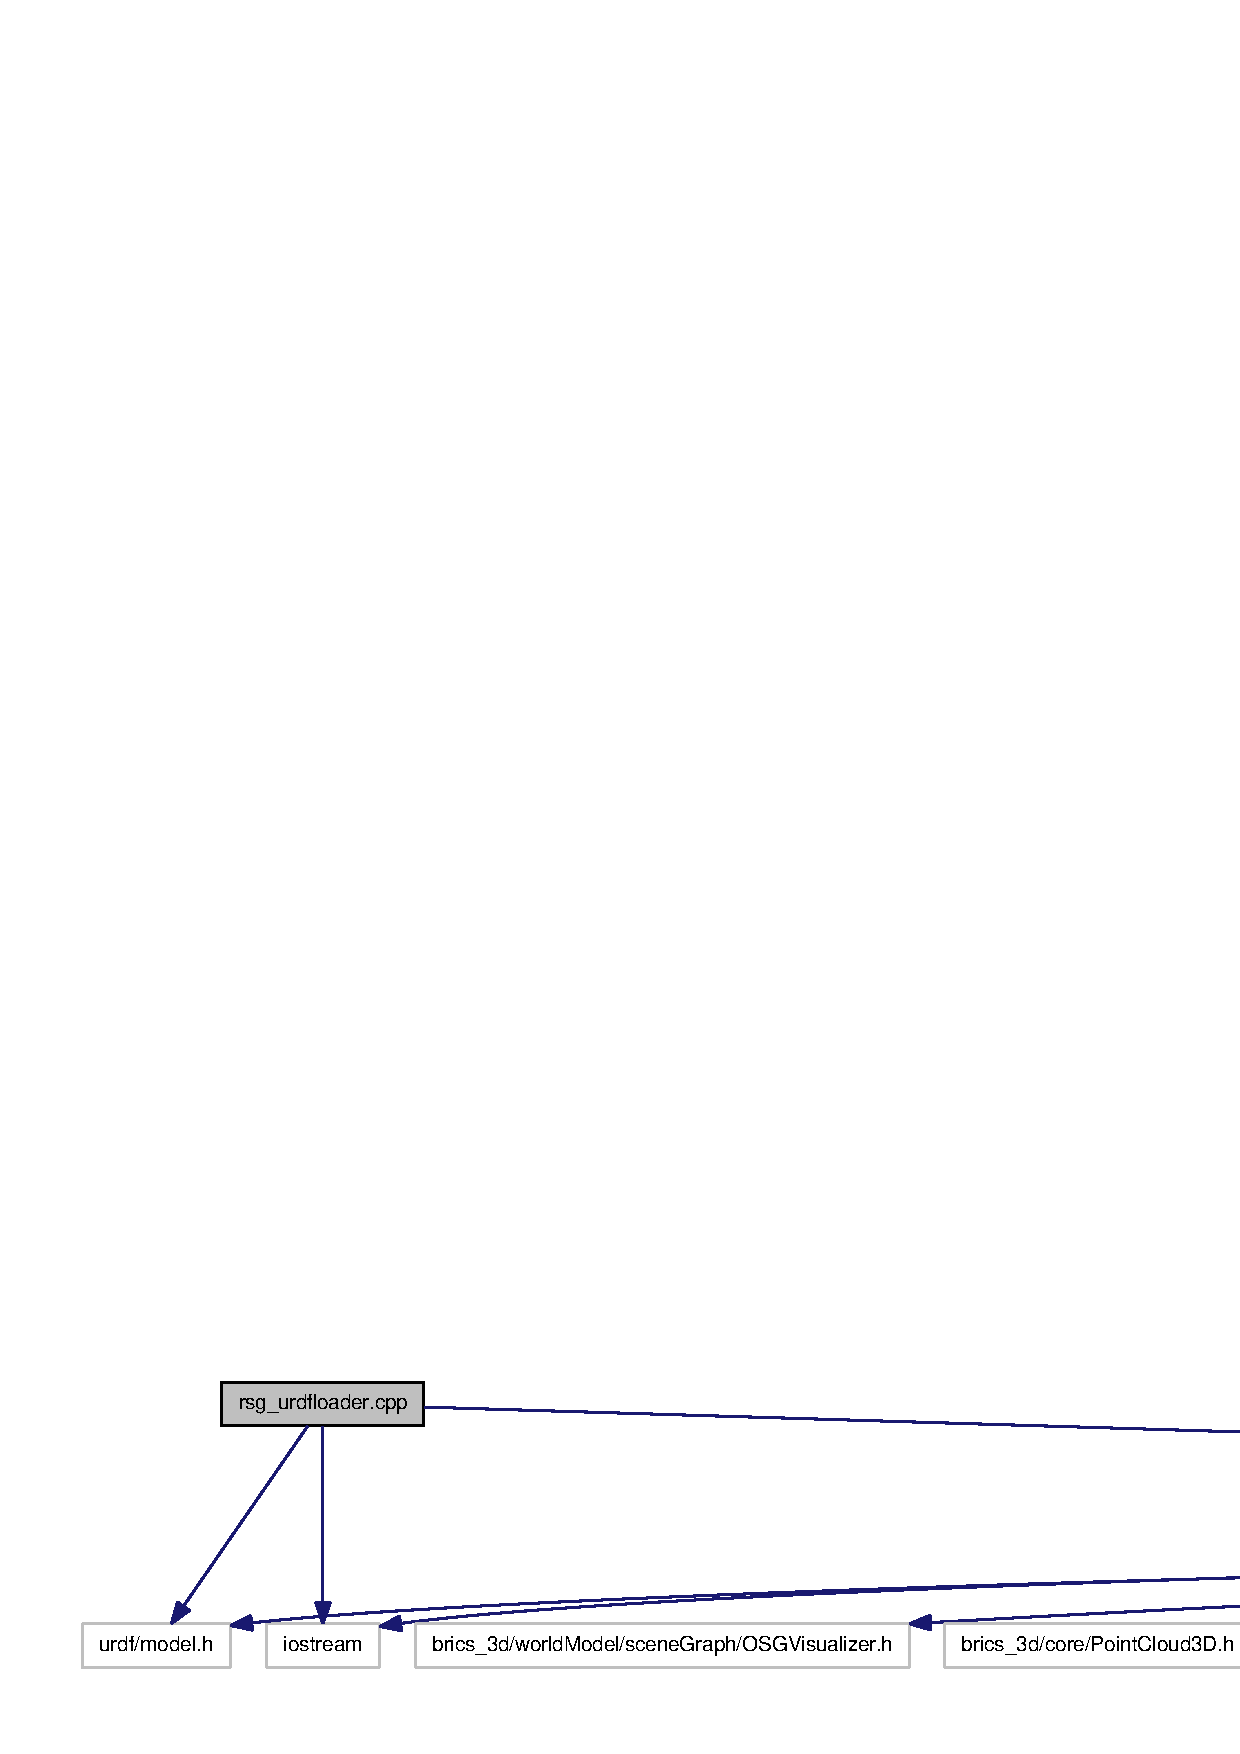
\includegraphics[width=350pt]{rsg__urdfloader_8cpp__incl}
\end{center}
\end{figure}
\subsection*{\-Functions}
\begin{DoxyCompactItemize}
\item 
int {\bf main} (int argc, char $\ast$$\ast$argv)
\end{DoxyCompactItemize}


\subsection{\-Function \-Documentation}
\index{rsg\-\_\-urdfloader.\-cpp@{rsg\-\_\-urdfloader.\-cpp}!main@{main}}
\index{main@{main}!rsg_urdfloader.cpp@{rsg\-\_\-urdfloader.\-cpp}}
\subsubsection[{main}]{\setlength{\rightskip}{0pt plus 5cm}int {\bf main} (
\begin{DoxyParamCaption}
\item[{int}]{argc, }
\item[{char $\ast$$\ast$}]{argv}
\end{DoxyParamCaption}
)}\label{rsg__urdfloader_8cpp_a3c04138a5bfe5d72780bb7e82a18e627}


\-Definition at line 126 of file rsg\-\_\-urdfloader.\-cpp.


\section{rsg\-\_\-urdfloader.\-h \-File \-Reference}
\label{rsg__urdfloader_8h}\index{rsg\-\_\-urdfloader.\-h@{rsg\-\_\-urdfloader.\-h}}
{\ttfamily \#include $<$string$>$}\*
{\ttfamily \#include $<$urdf\-\_\-model/model.\-h$>$}\*
{\ttfamily \#include $<$urdf/model.\-h$>$}\*
{\ttfamily \#include $<$tinyxml.\-h$>$}\*
{\ttfamily \#include $<$ros/console.\-h$>$}\*
{\ttfamily \#include $<$iostream$>$}\*
{\ttfamily \#include $<$brics\-\_\-3d/util/\-O\-S\-G\-Point\-Cloud\-Visualizer.\-h$>$}\*
{\ttfamily \#include $<$brics\-\_\-3d/util/\-O\-S\-G\-Triangle\-Mesh\-Visualizer.\-h$>$}\*
{\ttfamily \#include $<$brics\-\_\-3d/world\-Model/scene\-Graph/\-O\-S\-G\-Visualizer.\-h$>$}\*
{\ttfamily \#include $<$brics\-\_\-3d/core/\-Point\-Cloud3\-D.\-h$>$}\*
{\ttfamily \#include $<$brics\-\_\-3d/core/\-Logger.\-h$>$}\*
{\ttfamily \#include $<$brics\-\_\-3d/core/\-Homogeneous\-Matrix44.\-h$>$}\*
{\ttfamily \#include $<$brics\-\_\-3d/core/\-Triangle\-Mesh\-Implicit.\-h$>$}\*
{\ttfamily \#include $<$brics\-\_\-3d/core/\-Triangle\-Mesh\-Explicit.\-h$>$}\*
{\ttfamily \#include $<$brics\-\_\-3d/algorithm/filtering/\-Octree.\-h$>$}\*
{\ttfamily \#include $<$brics\-\_\-3d/algorithm/filtering/\-Box\-R\-O\-I\-Extractor.\-h$>$}\*
{\ttfamily \#include $<$brics\-\_\-3d/algorithm/registration/\-Iterative\-Closest\-Point\-Factory.\-h$>$}\*
{\ttfamily \#include $<$brics\-\_\-3d/algorithm/mesh\-Generation/\-Delaunay\-Triangulation\-O\-S\-G.\-h$>$}\*
{\ttfamily \#include $<$brics\-\_\-3d/world\-Model/\-World\-Model.\-h$>$}\*
{\ttfamily \#include $<$brics\-\_\-3d/world\-Model/scene\-Graph/\-Mesh.\-h$>$}\*
{\ttfamily \#include $<$brics\-\_\-3d/world\-Model/scene\-Graph/\-Box.\-h$>$}\*
{\ttfamily \#include $<$brics\-\_\-3d/world\-Model/scene\-Graph/\-Cylinder.\-h$>$}\*
{\ttfamily \#include $<$brics\-\_\-3d/world\-Model/scene\-Graph/\-Dot\-Graph\-Generator.\-h$>$}\*
{\ttfamily \#include $<$assimp/\-Importer.\-hpp$>$}\*
{\ttfamily \#include $<$assimp/scene.\-h$>$}\*
{\ttfamily \#include $<$assimp/postprocess.\-h$>$}\*
\-Include dependency graph for rsg\-\_\-urdfloader.\-h\-:
\nopagebreak
\begin{figure}[H]
\begin{center}
\leavevmode
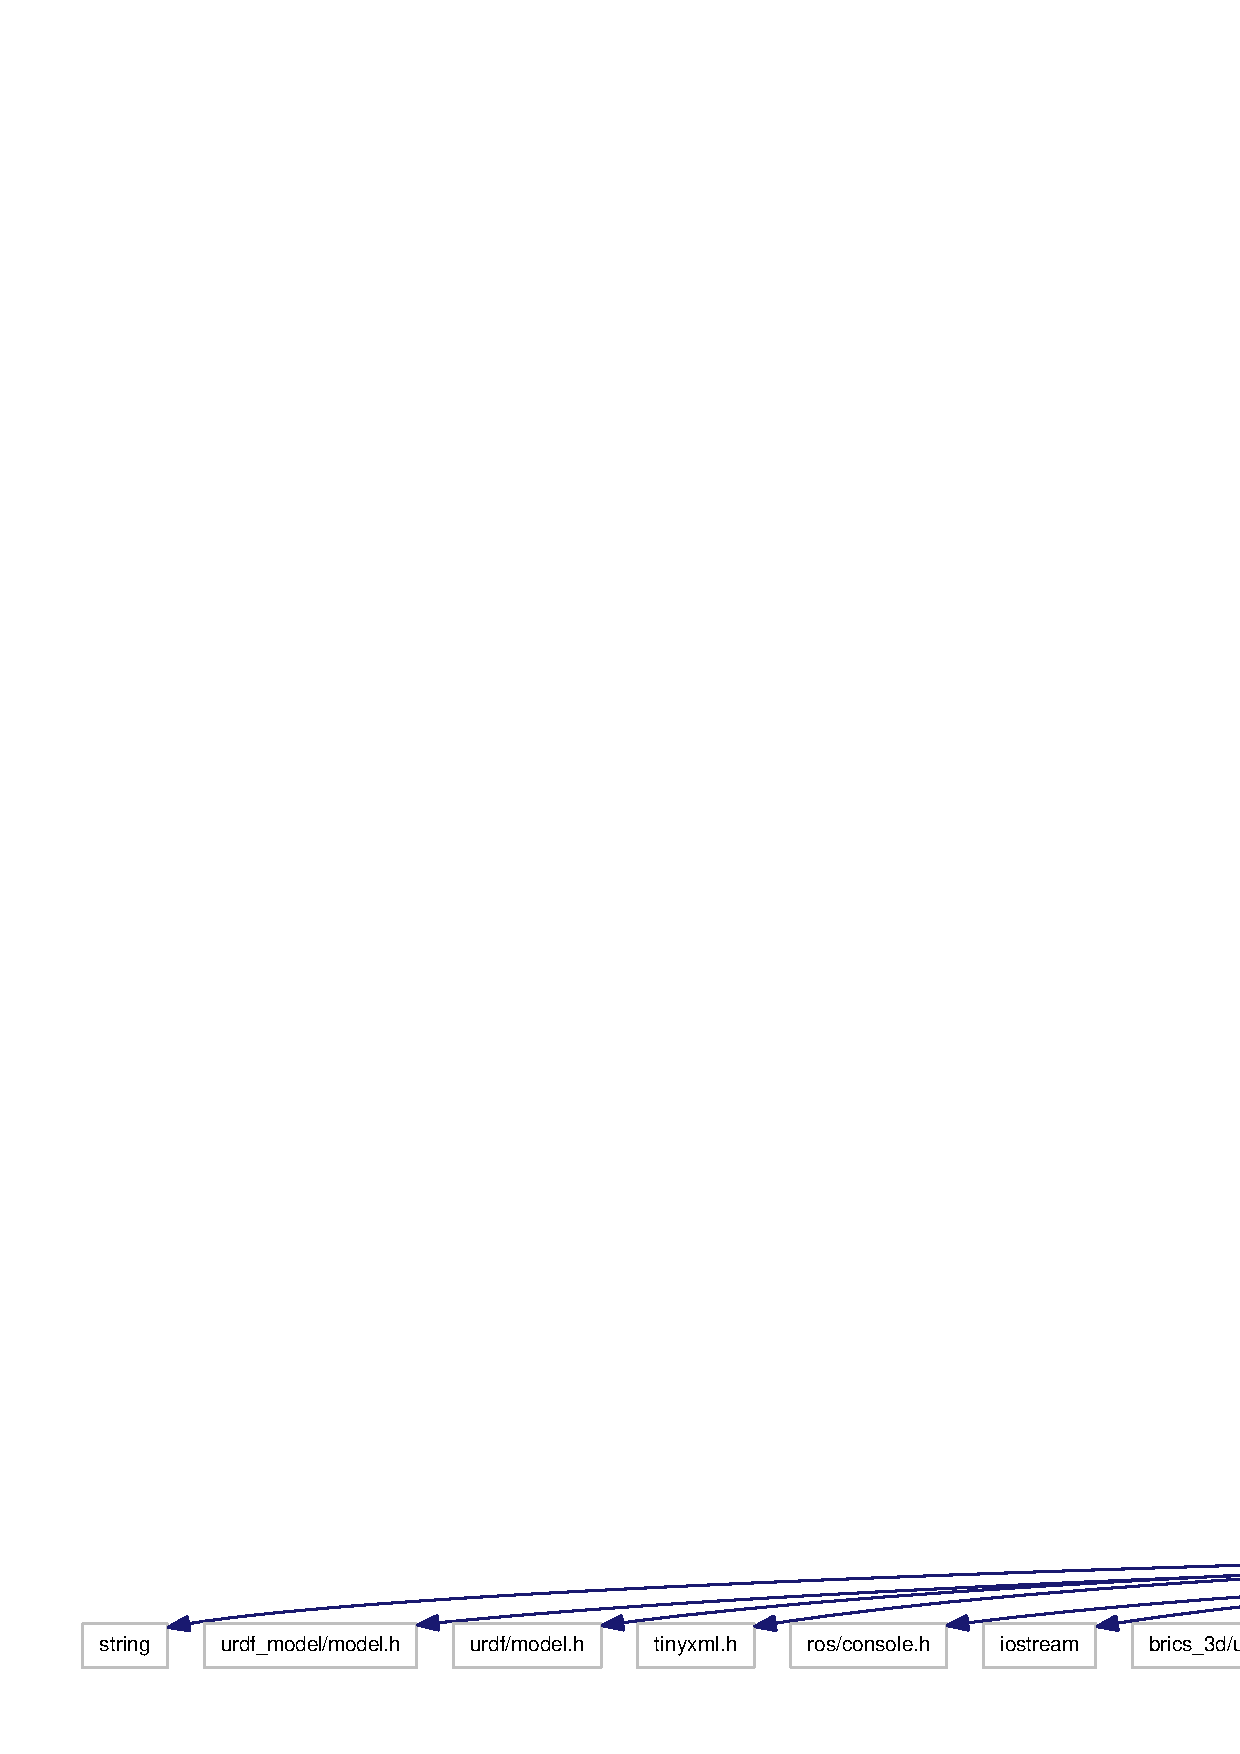
\includegraphics[width=350pt]{rsg__urdfloader_8h__incl}
\end{center}
\end{figure}
\-This graph shows which files directly or indirectly include this file\-:\nopagebreak
\begin{figure}[H]
\begin{center}
\leavevmode
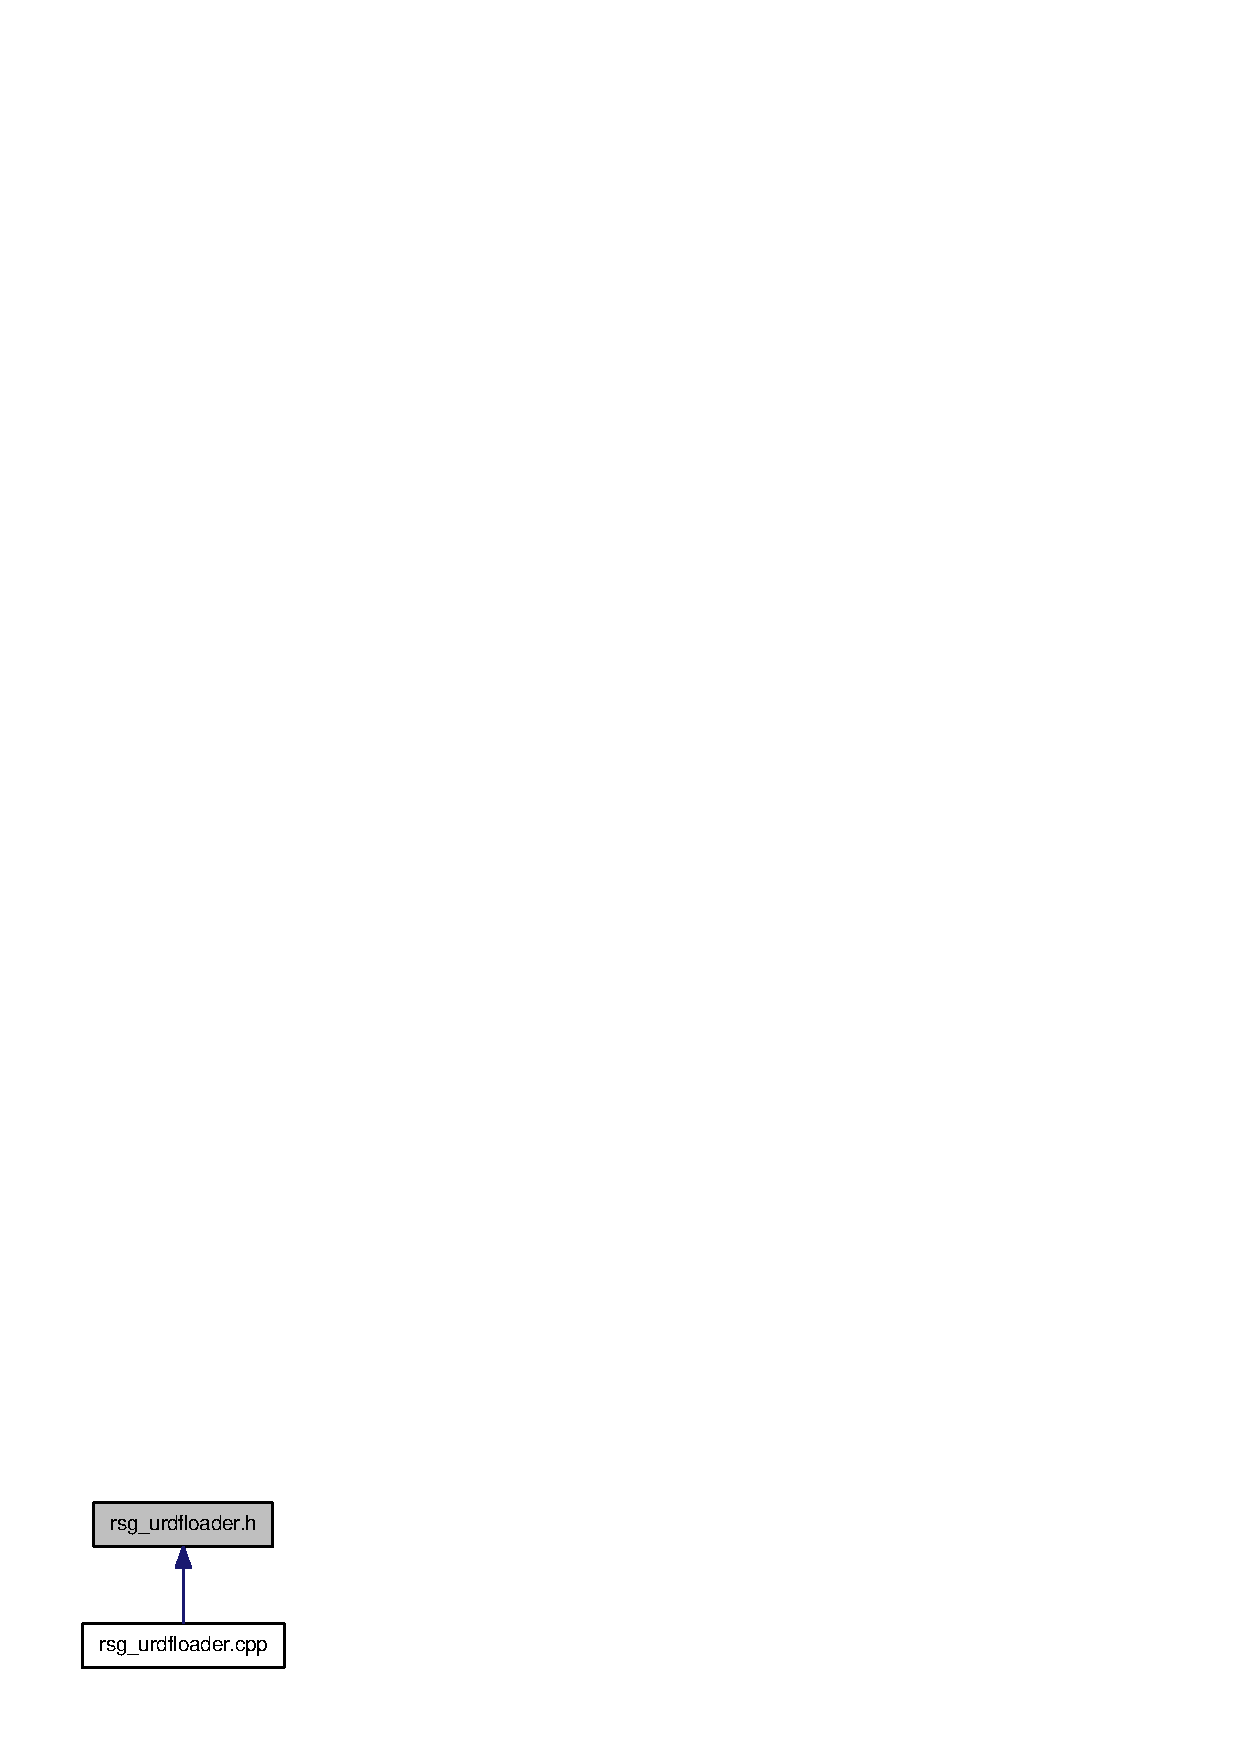
\includegraphics[width=140pt]{rsg__urdfloader_8h__dep__incl}
\end{center}
\end{figure}
\subsection*{\-Classes}
\begin{DoxyCompactItemize}
\item 
class {\bf rsg\-\_\-urdfloader\-::\-U\-R\-D\-Fto\-R\-S\-G}
\end{DoxyCompactItemize}
\subsection*{\-Namespaces}
\begin{DoxyCompactItemize}
\item 
namespace {\bf rsg\-\_\-urdfloader}
\end{DoxyCompactItemize}

\section{test.\-cpp \-File \-Reference}
\label{test_8cpp}\index{test.\-cpp@{test.\-cpp}}

\printindex
\end{document}
